\documentclass{sig-alternate}

\usepackage{amsmath}
\usepackage{graphicx}
\usepackage{subfigure}
\usepackage{color}
\usepackage{xspace}
\usepackage{url}
 \usepackage[utf8]{inputenc}

 % lorem
\newcommand{\lorem}               {\textcolor{green}{Lorem ipsum dolor sit amet, consectetur adipisicing elit, sed do eiusmod tempor incididunt ut labore et dolore magna aliqua. Ut enim ad minim veniam, quis nostrud exercitation ullamco laboris nisi ut aliquip ex ea commodo consequat. Duis aute irure dolor in reprehenderit in voluptate velit esse cillum dolore eu fugiat nulla pariatur. Excepteur sint occaecat cupidatat non proident, sunt in culpa qui officia deserunt mollit anim id est laborum.}}

% reviews
\newcommand{\thomas}[1]             {\textcolor{blue}{[Thomas] #1}}
\newcommand{\javier}[1]             {\textcolor{purple}{[Javier] #1}}
\newcommand{\keoma}[1]              {\textcolor{cyan}{[Keoma] #1}}
\newcommand{\remy}[1]               {\textcolor{yellow}{[Remy] #1}}
\newcommand{\jonathan}[1]           {\textcolor{pink}{[Jonathan] #1}}

% shortcuts
\newcommand{\name}                  {PEACH\xspace}
\newcommand{\smip}                  {SmartMesh~IP\xspace}

\graphicspath{{figures/}}

\begin{document}
\title{Feedbacks from a real-world low-power wireless sensor network deployment}

\numberofauthors{5}
\author{
  \alignauthor Brun-Laguna Keoma\\
    \affaddr{Inria, EVA team, Paris, France}\\
    \email{keoma.brun@inria.fr}
  \alignauthor Vilajosana Javier\\
    \affaddr{Universitat Oberta de Catalunya, Barcelona, Catalonia, Spain}\\
    \email{xvilajosana@uoc.edu}
  \alignauthor Léone Rémy \\
    \affaddr{Inria, EVA team, Paris, France}\\
    \email{remy.leone@inria.fr}
  \and
  \alignauthor Muñoz Jonathan\\
    \affaddr{Inria, EVA team, Paris, France}\\
    \affaddr{Gridbee, France}\\
    \email{jonathan.munoz@inria.fr}
  \alignauthor Watteyne Thomas \\
    \affaddr{Inria, EVA team, Paris, France}\\
    \email{thomas.watteyne@inria.fr}
}

\maketitle

\begin{abstract}
\lorem
\end{abstract}

\keoma{TODO:replace all images with .eps}

%==============================================================================
\section{Introduction}
\label{sec:intro}

% the PEACH project

Low temperatures have a very harmful impact on peach production as in 2013, 85\% of the production in the Mendoza region (western Argentina) was lost because of frost.
In April 2016, three research teams from different countries joined to start the deployment of a frost events prediction system~\cite{watteyne16peach}.
The goal of this project is to be able to precisely predict frost events and consequently reduce the impact of frost on peach production.
Frost detection systems already exist but few are actually able to propose prediction.

% the architecture

Due to the heavy machinery used to exploit the peach production, using cables is not conceivable.
The deployed solution is composed of a low-power wireless network and a back-end system to retrieve and visualize the data.
The network is formed by \smip devices from the Linear Technology company and is in charge of measuring the orchard environment, gather the data into a gateway and pass it to the back-end system.
The system collects both sensor values and network statistics.
The back-end system stores and backups the data and provide a visual interface and an API to access the data minutes after it was measured in Argentina.

% the deployment

The low-power wireless network is composed of 21 nodes uniformly distributed between the peach trees.
The covered area is an orchard with 204 trees on a 50*100m surface.
Each network mote is placed inside a water-tight box that is fixed on a 4m pole~\ref{fig:orchard}.
At the time of writing, the project is on its first stage.
During this stage, the goal is to verify that the network fulfill its requirements and that all the sensor values and statistics are correctly collected.
The location and environment of the current temperature sensors are not adequate, consequently, we do not exploit that information in this paper.
During the second stage, we will introduce additional sensors such as air temperature at different high, air relative humidity, soil moisture and soil temperature.

\begin{figure}
    \centering
    \includegraphics[width=\columnwidth]{orchard}
    \caption{The wireless motes deployed inside the orchard in Mendoza (Argentina)}
    \label{fig:orchard}
\end{figure}

\begin{figure*}
    \centering
    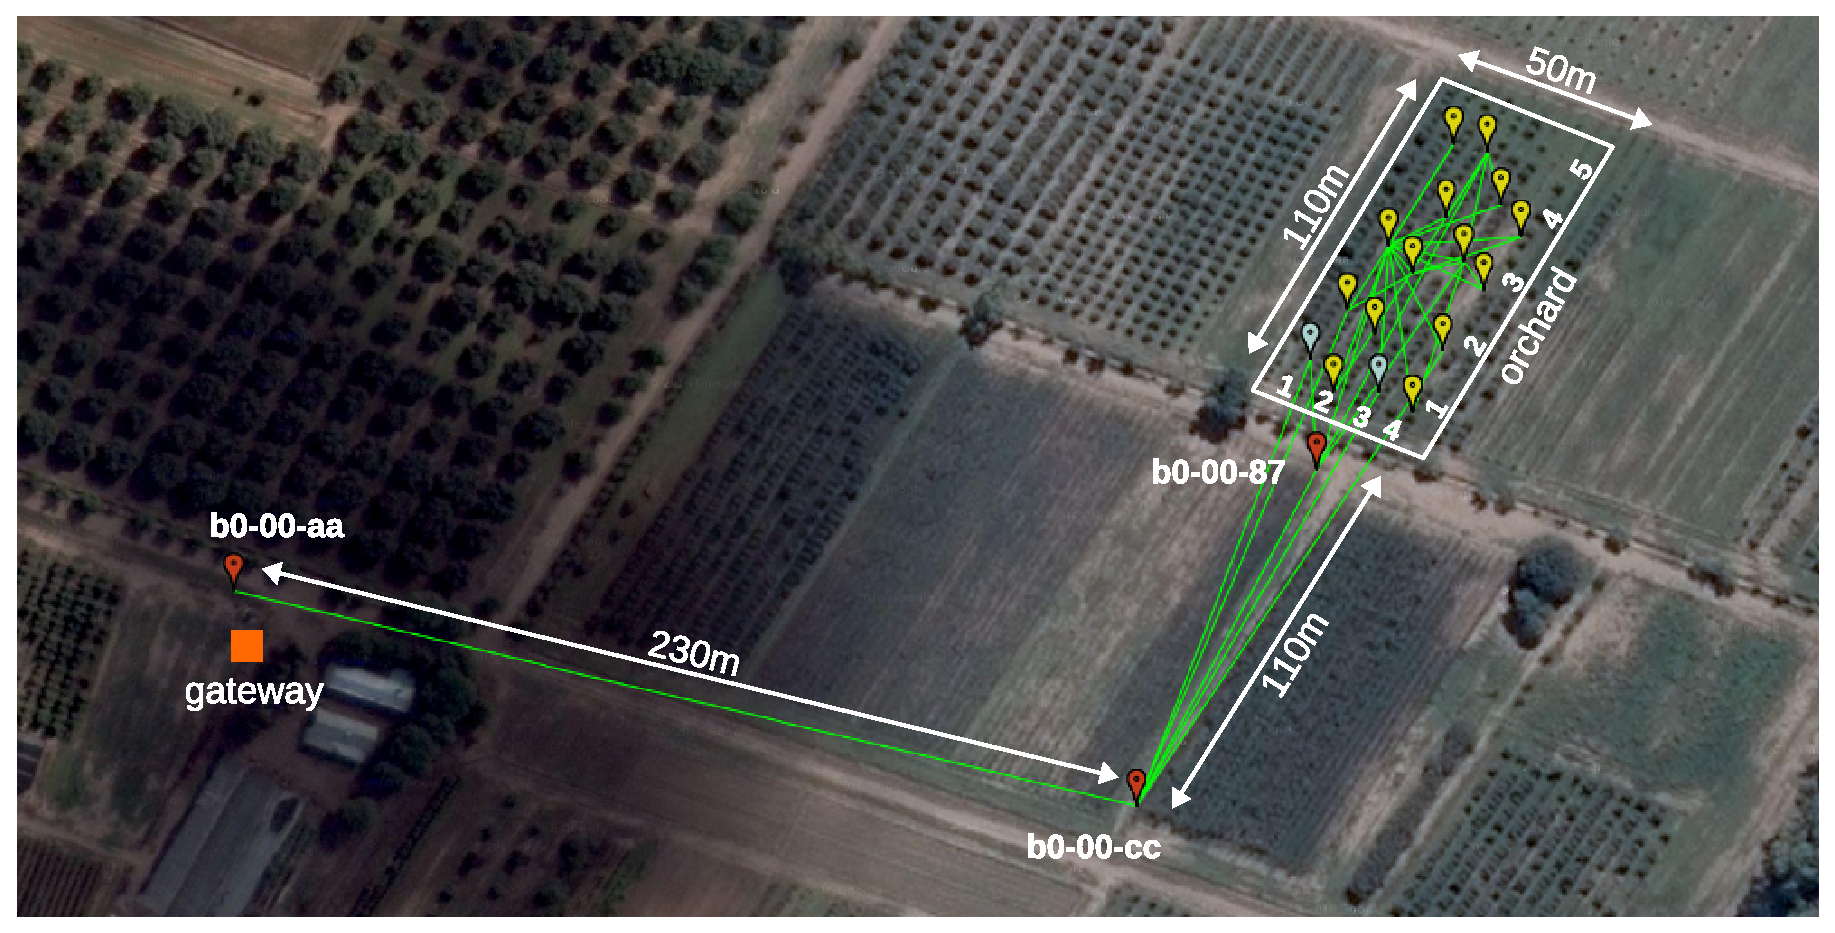
\includegraphics[width=\textwidth]{map_annotated}
    \caption{A map of the sensor deployed in the orchard near Mendoza (Argentina)}
    \label{fig:map}
\end{figure*}

% the hardware

We use four types of \smip devices to form the low-power wireless network~\ref{fig:map}.
The DC9018 with external antenna and the DC9003 with chip antenna are deployed inside the orchard.
Longe-range modes \thomas{To replace with exact name} are deployed outside the orchards to connect the network with the DC2274 device that is the gateway.

% the technology

The \smip motes are based on the IEEE 802.15.4e standard~\cite{std_ieee802154e} that includes a channel hopping mechanism to reduce the impact of multipath fading.
Channel hopping exploit the frequency diversity to reduce the probability of interferences and improve link reliability.
This mechanism show good results in the Wireless Sensor Network (WSN) context~\cite{watteyne2010mitigating, watteyne2009reliability} and allows to achieve high reliability while saving energy.

% the data

Each mote produce a temperature value every 30 seconds and network statistics, called ``health-reports'', every 5~minutes.
In 3~months, we gathered more than 2M~temperature value, and more than 180K~network statistics.
The health reports produced by any mote contain information about the mote itself and also about its neighbors.
%65184 HR_DEVICE, 63245 HR_DISCOVERED and 50285 HR_NEIGHBORS


\lorem

% the goal of this paper

The goal of this paper is to present the first feedbacks we have from the 3-month-old project and the lessons we learned from deploying WSN in real environment.
This paper makes the following contributions:
\begin{itemize}
    \item{We analyse the link asymmetry and show that a link can be consider a symmetrical in certain conditions}
    \item{}
\end{itemize}


% paper organisation
This paper is organized as follow:
Section~\ref{sec:collected} gives an in-depth description of the data we collect.

\lorem

%==============================================================================
\section{Collected Data}
\label{sec:collected}

% health report description

Each device in the network produce both sensor data and network statistics.
Network statistics can be separated in \textbf{Events} and \textbf{Health Reports} messages.
The Events messages are non periodic information triggered for instance when a node join the network or when a link (layer 2) is created/deleted.
The Health Report (HR) message are sent periodically and provide counters and statistics to assess the overall network health.
There are three types of HR:
\begin{itemize}
  \item HR\_DEVICE give information about the mote itself
  \item HR\_NEIGHBORS give information about the mote active neighbors
  \item HR\_DISCOVERED give information about the mote potential neighbors
\end{itemize}
Each device sends one type of Health Report every 5~min making the complete set of Health Report generated every 15~min.

%------------------------------------------------------------------------------
\subsection{HR\_DEVICE}

\keoma{should we actually put all the technical details here ?}
An HR\_DEVICE message contains the following fields:\\
\begin{tabular}{l|p{6cm}}
    field name      & description\\
    \hline
    charge          & node charge in mC\\
    queueOcc        & mean and max queue occupancy.\\
    temperature     & built-in temperature sensor value in C\\
    batteryVoltage  & node battery voltage in mV\\
    numTxOk         & number of packets sent from NET to MAC\\
    numTxFail       & number of packets not sent due to congestion or failure to allocate a packet\\
    numRxOk         & number of packets received\\
    numRxLost       & number of packets lost (discarded by NET layer due to misc errors)\\
    numMacDropped   & number of packets dropped by MAC (due to retry count or age or no route)\\
    numTxBad        & transmit failure counter for bad link\\
    badLinkFrameId  & frame id of link with the worst performance over the last health report interval\\
    badLinkSlot     & slot of link with the worst performance over the last health report interval\\
    badLinkOffset   & offset of link with the worst performance over the last health report interval\\
\end{tabular}

% HR_DISCOVERED

\lorem

% HR_NEIGHBORS

\lorem

%==============================================================================
\section{Link Symmetry}
\label{sec:symmetry}

% RSSI expectations

The Received Signal Strength Indication (RSSI) values can be retrieved from both active neighbors and discovered neighbors Health Reports, thus every 15~min for each pair of device.
Those RSSI values are averaged values over the 16 channels defined in the IEEE 802.15.4 standard~\cite{std_ieee802154_2011}.
In the rest of that paper we will use RSSI to denote the average RSSI over the 16 channels.

% environment

The peach orchard is located in a rural area that is not exposed to high traffic on the ISM band so we do not expect important external interferences.
Heavy machinery is used inside the orchard by farmers approximately every 20 days and during a period of one to two hours.
Those movements could create internal interferences such as multipath fading.

% symmetry analysis

A common assumption is to assume that a layer 2 link between two identical wireless nodes is asymmetrical.
We looked at the links statistics between the 18th of June and the 4th of July (16 days) and analysed the difference between the RSSI values.
The sample contains 411132 HR\_NEIGHBORS messages and concern 14 nodes with same hardware (DC9003).
During that period, 21 different bidirectional links are active with at least 50 transmissions.
For each of those links, we compute the RSSI difference for the two directions of the link (i.e from A to B and from B to A) and present the results in Fig.~\ref{fig:tab_symmetry}).
The very low RSSI difference shows that the links are very symmetrical.
Note that the RSSI is an average over the different channels.

\begin{figure}
    \centering
    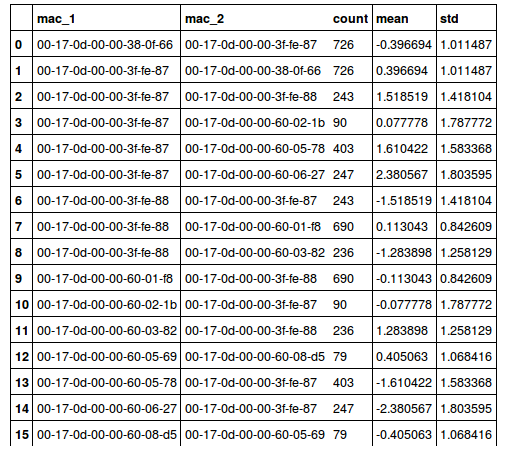
\includegraphics[width=\columnwidth]{tab_symmetry}
    \caption{The different active links between 2016-06-18 and 2016-06-25}
    \label{fig:tab_symmetry}
\end{figure}


%------------------------------------------------------------------------------
\section{Link Stability}

\lorem

\begin{figure}
    \centering
    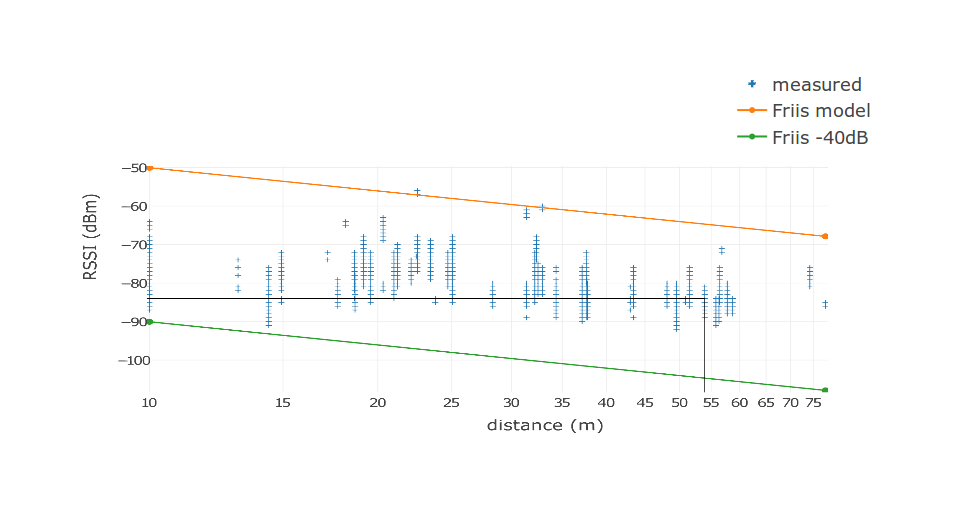
\includegraphics[width=\columnwidth]{pister_hack}
    \caption{The famous Pister-Hack model here}
    \label{fig:pister_hack}
\end{figure}

%------------------------------------------------------------------------------
\subsection{RSSI Threshold}

\lorem

\begin{figure}
    \centering
    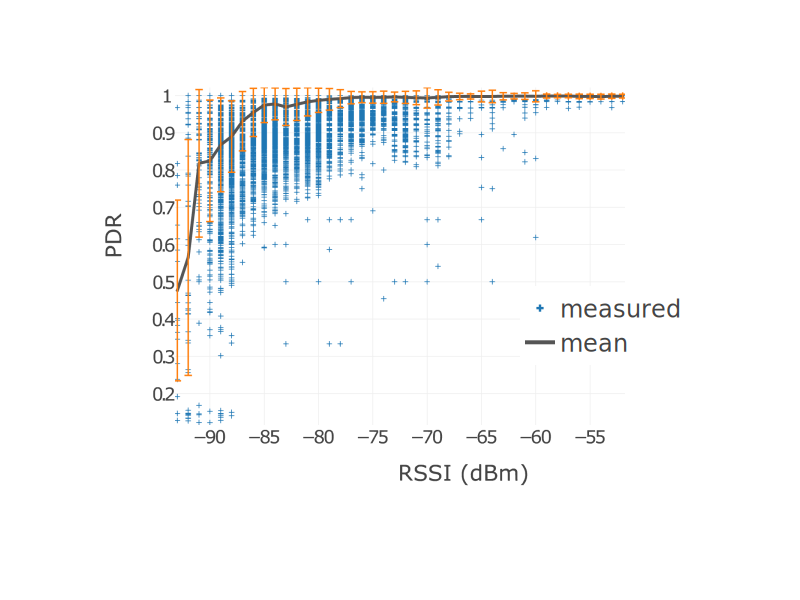
\includegraphics[width=\columnwidth]{waterfall}
    \caption{The PDR/RSSI waterfall}
    \label{fig:waterfall}
\end{figure}

%==============================================================================
\section{Topology}
\label{sec:topology}

% topology expectations

\lorem

% what we found

\lorem

\begin{figure}
    \centering
    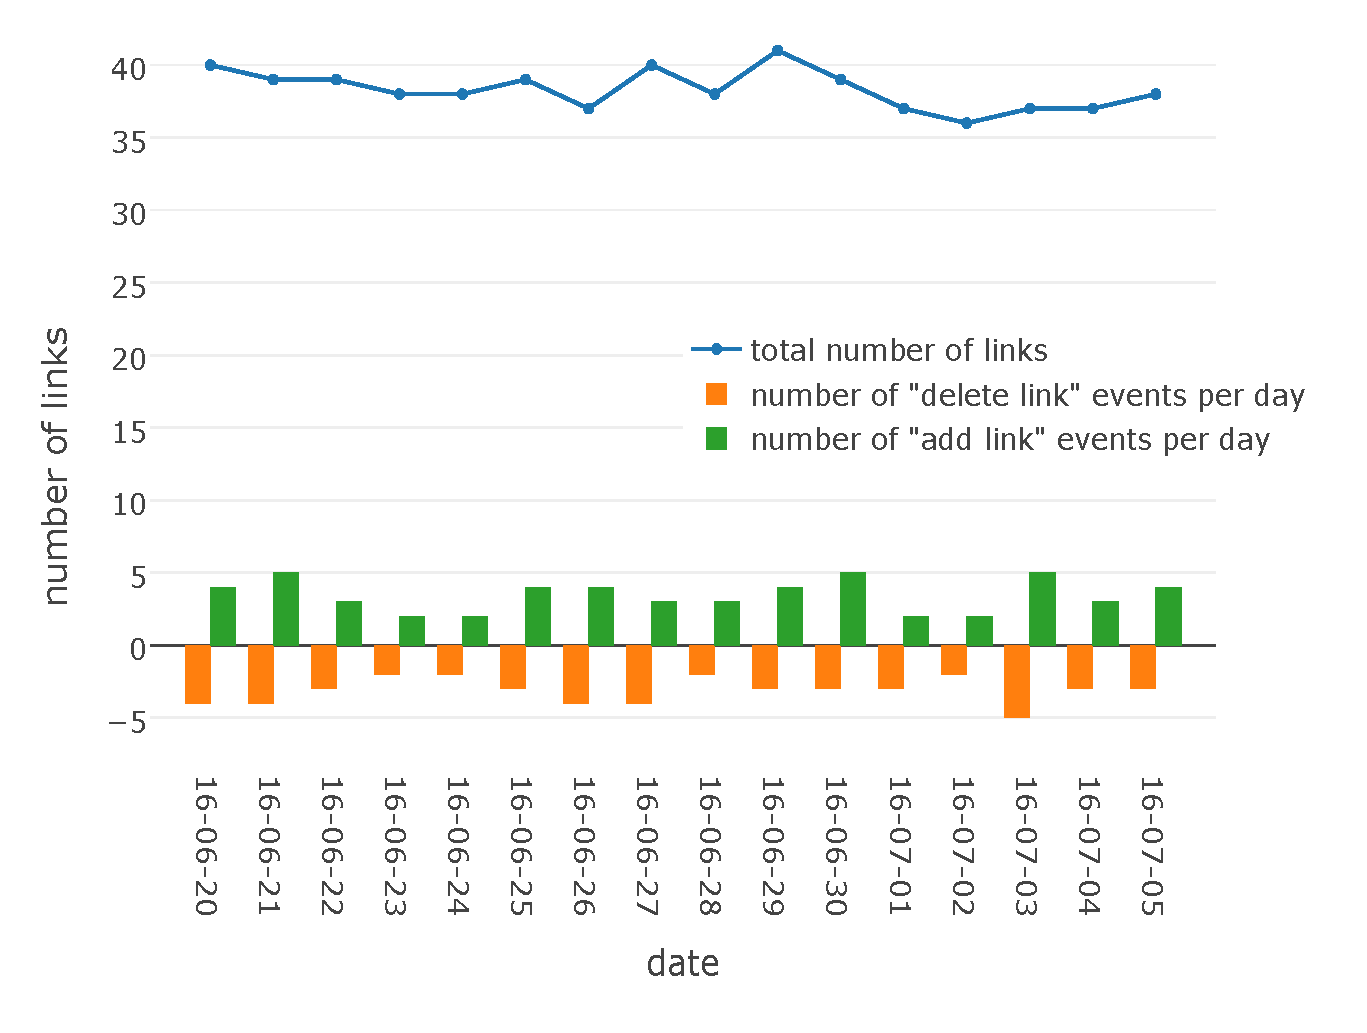
\includegraphics[width=\columnwidth]{net_churn}
    \caption{Network churn here}
    \label{fig:net_churn}
\end{figure}

%==============================================================================
\section{Charge}
\label{sec:charge}

% charge expectation

\lorem

\begin{figure}
    \centering
    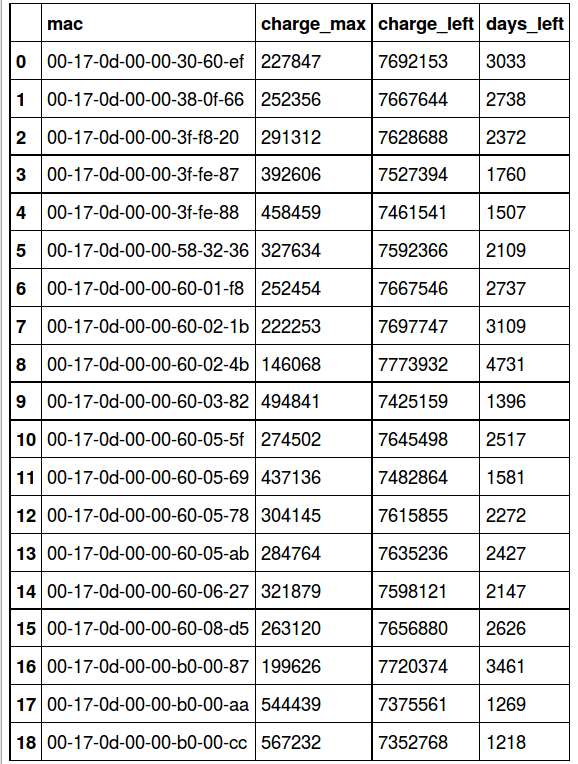
\includegraphics[width=\columnwidth]{stats_charge}
    \caption{The charge stats here}
    \label{fig:stats_charge}
\end{figure}

%==============================================================================
\section{Reliability}
\label{sec:reliability}

% reliability expectation

\lorem

\begin{figure}
    \centering
    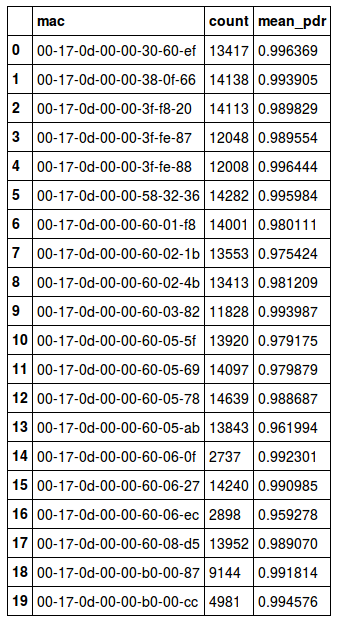
\includegraphics[width=\columnwidth]{stats_reliability}
    \caption{The reliability stats here}
    \label{fig:stats_reliability}
\end{figure}

%==============================================================================
\section{Conclusion}
\label{sec:conclusion}

% conclusion

\lorem

%==============================================================================

\bibliographystyle{abbrv}
\bibliography{16chants}

\end{document}

%
